\documentclass[12pt,b5paper,twoside,openright]{book}
\usepackage{blindtext}
\usepackage{microtype}
\usepackage{listings}
\usepackage{color}
\usepackage{enumerate}
\usepackage{caption}
\usepackage{amsmath}
\usepackage{float}
\usepackage{algorithm}% http://ctan.org/pkg/algorithm
\usepackage{algpseudocode}% http://ctan.org/pkg/algorithmicx
\usepackage{graphicx}

\renewcommand{\chaptername}{Bab}
\renewcommand{\contentsname}{Daftar Isi}
\renewcommand{\listfigurename}{Daftar Gambar}
\renewcommand{\listtablename}{Daftar Tabel}
\renewcommand{\figurename}{Gambar}
\renewcommand{\tablename}{Tabel}
\usepackage{imakeidx}
\makeindex[columns=2, title=Indek,options= -s example_style.ist]

\usepackage{fancyhdr}
\pagestyle{fancy}
\fancyhf{}
\fancyhead[LE]{\rightmark}
\fancyhead[RO]{\leftmark}
\fancyfoot[LE,RO]{\thepage}
 
\renewcommand{\headrulewidth}{1pt}
%\renewcommand{\footrulewidth}{1pt}
\pagenumbering{roman}


\usepackage{draftwatermark}
\SetWatermarkText{DRAFT}
\SetWatermarkScale{5}
\SetWatermarkColor[gray]{0.95}
 

\begin{document}
%% for code snippet
\definecolor{dkgreen}{rgb}{0,0.6,0}
\definecolor{gray}{rgb}{0.5,0.5,0.5}
\definecolor{mauve}{rgb}{0.58,0,0.82}
\lstset{frame=tb,
  language=Java,
  aboveskip=3mm,
  belowskip=3mm,
  showstringspaces=false,
  columns=flexible,
  basicstyle={\small\ttfamily},
  numbers=left,
  numberstyle=\small\ttfamily\color{black},
  keywordstyle=\color{blue},
  commentstyle=\color{dkgreen},
  stringstyle=\color{mauve},
  breaklines=true,
  breakatwhitespace=true,
  tabsize=3
}

\title{{ Bagaiamana Berfikir Seperti Imuwan Komputer}}
\author{Allen Downey \\Diterjemahkan oleh Tim Buku Prodase - Universitas Telkom}

\date{}

\maketitle
\newpage
\frontmatter
\tableofcontents
\addcontentsline{toc}{chapter}{Daftar Tabel}
\listoftables
\addcontentsline{toc}{chapter}{Daftar Gambar}
\listoffigures


\mainmatter
%%%%%%%%%%%%%%%%ISI BUKU%%%%%%%%%%%%%%%%%%%%%%%
\chapter{Cara Program}
Tujuan dari buku ini adalah mengajarkan kepada kamu bagaimana berfikir seperti seorang ilmuan komputer. Saya sangat suka bagaimana seorang ilmuan komputer berfikir karena mereka menggabungkan aspek-aspek terbaik dari ilmu Matematika, ilmu Teknik, dan ilmu pengetahuan alam. Sebagaimana halnya Matematikawan, ilmuan komputer menggunakan bahasa formal untuk menyatakan ide khususnya yang berkenaan dengan komputasi. Seperti Insinyur(\textit{Engineer}), ilmuan komputer juga merancang sesuatu, merangkai beberapa komponen kedalam sebuah sistem dan mengeveluasi kelebihan dan kekurangan dari berbagai alternatif solusi. Mirip dengan ilmuan pada umumnya, para ilmuan komputer melakukan observasi tingkah laku dari sistem yang kompleks, membentuk beberap hipotesis dan menguji prediksi yang mereka buat.

Satu-satunya keahlian yang paling penting bagi seorang ilmuan komputer adalah keahlian dalam memecahkan masalah (\textit{problem-solving}). Yang saya maksudkan dengan kemampuan memecahkan masalah adalah kemampuan mereka dalam melakukan formulasi masalah, berfikir secara kreatif mengenai solusi dari masalah yang telah diformulasikan dan mengekspresikan sebuah solusi secara jelas dan akurat.  Dan ternyata proses yang kamu lalui ketika belajar program komputer  adalah sebuah kesempatan yang istimewa  dalam berlatih keahlian memecahkan masalah. Itu kenapa judul dari bab ini adalah "Cara Program".

Pada satu sisi kamu akan belajar pemrograman, yang mana merupkah keahlian yang sangat penting. Disisi lainya, kamu akan menggunakan pemrograman sebagai sarana untuk belajar 

\section{Apa itu bahasa pemrograman?}

Bahasa pemrograman yang akan kamu \textbf pelajari adalah Java, yang termasuk sebuah bahasa pemrograman yang relatif baru (Dirilis pertama kali oleh Sun Microsystem pada may 1995). Java adalah salah satu contoh dari bahasa pemrograman level tinggi (\textit{high-level language}); bahasa pemrograman lain yang juga termasuk kategori bahasa pemrograman level tinggi adalah bahasa Python, C atau C++ dan Perl.

Selain istilah bahasa pemrograman level tinggi, terdapat juga istilah bahasa pemrograman level rendah (\textit{low level languages}) dan terkadang dikenal juga dengan istilah bahasa mesin atau bahasa \textit{assembly}. Pada kenyataanya, komputer hanya bisa memahami bahasa pemrograman level rendah. Oleh sebab itu, sebuah program yang ditulis menggunakan bahasa level tinggi harus diterjemahkan terlebih dahulu ke bentuk bahasa level rendah sebelum program tersebut dijalankan. Proses penterjemahan ini membutuhkan waktu sebelum bisa dijalankan oleh komputer, hal ini menjadi salah satu kekurangan dari bahasa pemrograman level tinggi.

Keunggulan dari bahasa  level-tinggi cukup banyak jika dibandingkan dengan kekuranganna. Pertama, jauh lebih mudah untuk membuat program dengan menggunakan bahasa level-tinggi; waktu yang dibutuhkan untuk menuliskan program jauh lebih singkat, penulisannya juga jauh lebih pendek dan mudah dibaca jika dibandingkan dengan bahasa level-rendah. Keuntungan yang kedua adalah portabilitas dalam menjalankannya diberbagai macam arsitektur komputer dengan tanpa modifikasi. Berbeda halnya dengan program yang ditulis dengan bahasa level-rendah yang hanya bisa dijalankan di komputer tertentu, sehingga perlu dimodifikasi jika ingin dijalankan pada komputer dengan arsitektur yang berbeda.

Oleh karena kelebiha-kelebihan tersebut, maka hampir semua program ditulis dengan menggunakan bahasa pemrograman level-tinggi. Bahasa level-rendah hanya digunakan untuk membuat program-program tertentu saja yang jumlahnya juga sedikit.

Terdapat dua cara untuk menterjemahkan sebuah program; \textbf{interpretasi} (\textit{interpreting}) dan \textbf{kompilasi} (\textit{compiling}). Sebuah \textit{interpreter} adalah sebuah program yang membaca sebuah program level-tinggi dan melakukan apa yang diminta oleh program tersebut. Sebagai akibatnya, interpreter akan menterjemahkan program baris demi baris
Sementara \textit{compiler} adalah sebuah program yang membaca sebuah program level-tinggi dan menterjemahkan keseluruhan program secara langsung, sebelum menjalankan perintah apa pun dari program tersebut. Sering kali, kamu akan melakukan proses kompilasi(\textit{compiling}) secara terpisah terlebih dahulu, kemudian baru  menjalankan (\textit{run}) program. Pada kasus ini, program level-tinggi disebut dengan istilah kode sumber (\textit{source code}) dan program yang telah diterjemahkan disebut dengan istilah kode objek (\textit{object code}) atau \textit{executable}.

Java adalah sebuah bahasa pemrograman yang menggunakan kompilasi dan juga interpretasi ketika menjalankan program. Alih-alih menterjemahkan program ke dalam bahasa mesin, \textit{Java compiler} mengubahnya ke dalam bentuk kode bita (\textit{byte code}). Sama halnya dengan bahasa mesin, kode bita sangat mudah dan juga cepat untuk diterjemahkan (interpretasi). Perbedaannya, kode bita tidak bergantung pada arsitektur komputer tertentu ( lebih \textit{portable}) seperti halnya bahasa level-tinggi. Artinya sebuah kode bita yang dihasilkan di sebuah komputer dapat dipindahkan dan dijalankan di komputer lain yang berbeda mesin/arsitektur. Kemampuan ini merupakan salah satu kelebihan dari bahasa Java jika dibandingkan dengan bahasa level-tinggi lainnya.

\begin{figure}[H]
	\centering 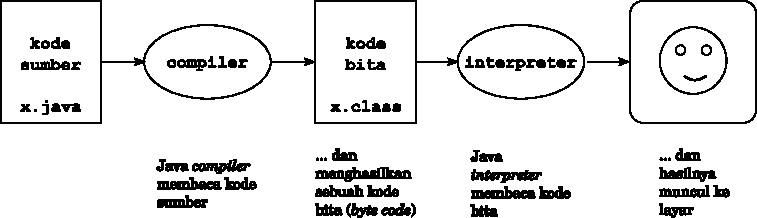
\includegraphics{images/compilingProcess.pdf}
	\caption{Proses kompilasi dan interpretasi pada bahasa Java}
	\label{fig:binaryTreeRekursif}
\end{figure}

Walaupun proses ini terlihat kompleks, namun di beberapa perangkat lunak (\textit{software}) yang digunakan untuk meprograman (sering disebut Integrated Development Environment/IDE) proses-proses tersebut telah dibuat otomatis untuk kamu. Sehingga kamu hanya cukup menekan sebuah tombol "run" saja, maka \textit{software} IDE tersebut akan melakukan kompilasi dan interpretasi untuk program yang kamu buat.Namun disisi lain, kamu tetap harus tahu langkah-langkah yang terjadi dibalik proses yang telah terotomatis tadi, agar ketika terjadi kesalahan maka kamu dapat dengan mudah mengetahui penyebabnya.

\section{Apa itu program?} 

Program adalah sebuah runtutan instruksi yang menyatakan bagaiman melakukan sebuah komputasi \footnote{Definisi ini tidak berlaku untuk seluruh bahasa pemrograman. Sebagai alternatif, lihat $http://en.wikipedia.org/wiki/Declarative\_programming$.}. Istilah komputasi bisa berarti sebagai sesuati yang matematis, seperti menyelesaikan sebuah sistem persamaan atau menemukan akar dari sebuah polinomial, tetapi bisa juga diartikan sebagai sebuah komputasi simbolik, seperti mencari dan mengganti teks pada sebuah dokumen atau mengkompilasi sebuah program. 

Instruksi atau yang sering disebut dengan statemen (\textit{statement}), memilik bentuk yang berbeda-beda untuk setiap bahasa pemrograman, namun terdapat beberapa instruksi dasar yang bisa dilakukan oleh seluruh bahasa pemrograman. instruksi-instruksi dasar tersebut antara lain:

\begin{enumerate}
	\item \textbf{masukan(\textit{input}):} instruksi-instruksi yang digunakan untuk mendapatkan data dari \textit{keyboard} atau sebuah berkas atau dari perangkat lain
	\item \textbf{keluaran (\textit{output}):} instruksi-instruksi yang digunakan untuk menampilkan data kelayar atau mengirimkannya ke berkas atau perangkat lainnya
	\item \textbf{matematika(\textit{math}): }instruksi-instruksi yang digunakan untuk melakukan operasi matematika seperti penjumlahan, pengurangan, perkalian, pembagian dan lainya
	\item \textbf{pengkondisian(\textit{testing}):} instruksi-instruksi yang digunakan untuk memeriksa kondisi tertentu dan menjalankan urutan statemen yang sesuai.
	\item \textbf{perulangan(\textit{repetition}):} instruksi-instruksi yang digunakan untuk melakukan pengulangan terhadap sebuah atau beberapa statemen.
\end{enumerate}

Setiap program yang pernah kamu gunakan, tidak peduli seberapa rumit apapun program tersebut, pasti tersusun dari kombinasi dari instruksi-instruksi dasar di atas. Oleh sebab itu, salah satu cara untuk menjelaskan pemrograman adalah sebagi sebuah proses yang memecah-mecah sebuah pekerjaan yang besar dan kompleks kedalam bentuk beberapa sub pekerjaan yang jauh lebih kecil secara terus menerus hingga sub pekerjaan tersebut dapat secara sederhana dijalankan dengan menggunakan salah satu instruksi-instruksi dasar tadi.

\section{Apa itu \textit{debugging}?}

Untuk alasan lelucon, error (keselahan) yang terdapat pada pemrograman disebut dengan "kutu" (\textit{bug}) dan proses yang dilakukan untuk menemukan dan memperbaik "kutu" tersebut dikenal dengan istilah \textit{debugging}.

Terdapat tiga jenis \textit{error} yang sering muncul dalam sebuah program yaitu \textit{syntax error}, \textit{run-time error} dan \textit{logic dan semantik error}. Penting dan sangat bermanfaat sekali bagi kamu jika kamu bisa membedakan ketiganya,  sehingga kamu dapat dengan cepat dan juga mudah dalam menelusuri kesalahan yang ada dan kemudian memperbaikinya.

\subsection{Kesalahan Sintak \textit{(Syntax Error)}}
\textit{Compiler} hanya bisa melakukan kompilasi jika kode program yang ditulis telah benar secara sintak, jika tidak maka proses kompilasi akan gagal dan kamu tidak akan dapat menjalankan program tersebut. Sintak berarti struktur dan juga aturan dari struktur penulisan dari kode program yang kamu buat.

Sebagai contoh, dalam bahasa inggris sebuah kalimat harus dimulai dengan huruf besar dan diakhiri dengan tanda titik. \\
\texttt{ini adalah contoh kalimat yang salah secara sintak.} \\
\texttt{Ini juga salah secara sintak}

Bagi kebanyakan pembaca, sedikit kesalahan sintak bukanlah masalah yang berarti. Sebagai contoh\textit{ kta msh bsa mmbaca dan memhami tlsan ini dngn baik} walaupu penulisan kata-katanya banyak yang tidak lengkap.

Kemampuan seperti itu tidak dimiliki oleh \textit{compiler}, jika terjadi satu satu kesalahan penulisan (sintak) di kode program yang kamu buat maka \textit{compiler} akan menampilkan pesan error \textit{error message} dan seketika itu akan menghentikan proses kompilasi. Ketika hal tersebut terjadi, maka program yang kamu buat bisa dipastikan tidak akan bisa dijalankan.

Lebih buruk lagi, dalam bahasa Java terdapat lebih banyak aturan sintak dibandingkan dengan sintak yang dimiliki oleh bahasa inggris atau bahasa lainnya, dan pesan error yang tampilkan sering sekali tidak terlalu membantu. Seiring bertambahnya pengalaman kamu, maka kamu akan membuat sedikit kesalahan dan akan lebih cepat dalam menemukannya.
\subsection{Kesalahan ketika menjalankan \textit{(Run-Time Error)}}
Jenis kesalahan berikutnya adalah kesalahan yang muncul ketika menjalankan program (\textit{Run-time Error}). Disebut seperti itu, karena kesalahan tersebut tidak muncul hingga program dijalankan. Di Java, sebuah \textit{run-time error} terjadi ketika \textit{interpreter} menjalankan kode bita (\textit{byte code}) dan terjadi kesalahan dalam proses tersebut.

Java adalah sebuah bahasa pemrograman yang cendrung aman, artinya seluruh potensi kesalahan diupayakan dapat dideteksi oleh \textit{compiler}. Sehingga \textit{run-time error} dapat diminimalisir, khususnya untuk program-program yang sederhana.

Di Java, \textit{run-time error} dikenal ddngan istilah \textit{exceptions}(pengecualian). Dan di banyak lingkungan, \textit{ecxeptions} muncul dalam bentuk \textit{windows} atau \textit{dialog box} yang berisi informasi mengenai apa yang telah terjadi dan apa yang program lakukan ketika hal tersebut terjadi. Informasi ini sangat berguna sekali ketika melakukan \textit{debugging}
\subsection{Kesalahan logika dan semantik \textit{(Logic errors and sematics)}} 
Jenis \textit{error} yang ketiga adalah kesalahan logika dan semantik. Jika program kamu memiliki kesalahan logika, maka program kamu akan dikompilasi dan dijalankan tanpa adanya \textit{error message}, namun tidak akan melakukan apa yang seharusnya. Melainkan akan melakukan hal yang lain. Lebih spesifiknya, program yang kamu buat tidak akan melakukan apa yang kamu perintahkan.

Masalahnya adalah program yang kamu tulis bukanlah program yang kamu inginkan. Hal ini terjadi karena semantik atau makna dari kode program yang kamu buat salah. Menemukan kesalahan logika pada sebuah program adalah hal yang cukup rumit karena kamu harus bekerja secara terbalik, dimulai dari mengidentifikasi keluaran dari program dan mencoba untuk menganalisa apa yang sebenarnya terjadi.

\subsection{Debugging}
Salah satu keahlian yang sangat penting kamu kuasai pada pelajaran ini adalah \textit{debugging}. Walaupun \textit{debugging} bisa jadi membuat kamu frustasi, namun ia merupakan hal yang sangat menarik dan menantang dan merupakan bagian yang sangat bernilai dalam pemrograman.

\textit{Debugging} mirip dengan pekerjaan detektif. Kamu berhadapan dengan petunjuk-petunjuk dan kamu harus menyimpulkan proses serta kejadian yang mengakibatkan hasil yang kamu lihat.

\textit{Debugging} juga serupa dengan ilmu eksperimental (\textit{experimental science}). Disaat kamu mendapati program yang kamu buat mengalami \textit{error}, maka kamu akan membuat semacam dugaan (hipotesis) yang menjadi penyebab dari \textit{error} tersebut, kemudian kamu memodifikasi kode program tersebut berdasarkan hipotesis yang kamu buat, dan kemudian kamu mencoba menjalankan ulang program kamu untuk membuktikan apakah hipotesis kamu benar/tidak. Jika hipotesis kamu benar, maka kamu dapat memprediksi hasil dari modifikasi kamu, dan kamu semakin dekat dengan program yang berfungsi dengan baik. Sebaliknya, jika hipotesis kamu salah, maka kamu harus membuat hipotesis baru untuk kemudian mengulangi proses sebelumnya. Hal ini akan berlangsung secara terus menerus hingga \textit{error} dari program kamu berhasil teratasi. Sebagaimana yang dikatakan oleh \textit{Sherlock Holmes}, "Ketika kamu telah mengeliminasi hal-hal yang tidak mungkin, apa pun yang tersisa walaupun mustahil, haruslah sebuah kebenaran" (dari A. Conan Doyle's \textit{The sign of Four.})

Bagi sebagian orang, pemrograman dan \textit{debugging} adalah hal yang sama. Karena pemrograman adalah sebuah proses \textit{debugging} yang bertahap dari sebuah program hingga program terebut menjalankan apa yang kamu inginkan. Idenya adalah bahwa kamu harus memualai dengan sebuah program yang bisa dijalankan untuk melakukan sesuatu, tidak peduli sekecil apapun yang bisa dilakukan. Kemudian tambahkan modifikasi kecil ke program tersebut diikuti dengan \textit{debugging}, sehingga dengan begitu kamu akan selalu memiliki sebuah program yang berjalan dengan baik dan program yang kamu buat makin lama akan semakin kompleks.

Sebagai contoh, Linux adalah sebuah sistem operasi yang terdiri dari ribuan baris kode program yang pada awalnya hanyalah sebuah program sederhana yang digunakan olen Linus Trovalds untuk mengeksplorasi \textit{chip} Intel 80396. Menurut Larry Greenfield, " Salah satu proyek pertama yang dikerjakan ole Linus adalah sebuah program yang mencetak secara bergantian tulisan AAAA dan BBBB. Kemudian program ini berevolusi menjadi Linux" (dari \textit{The Linux Users' Guide} Beta Version 1).

Pada bab berikutnya, saya menambahkan lebih banyak saran mengenai \textit{debugging} dan praktik-prakatik pemrograman lainnya.


\section{Bahasa Formal dan Bahasa Alami}

Bahasa alami adalah bahasa-bahasa yang digunakan oleh orang-orang untuk berbicara, contohnya seperti bahasa Inggris,Spanyol dan Prancis. Bahasa tersebut tidak dirancang oleh manusia, namun berevolusi secara alami.

Bahasa formal adalah bahasa yang dirancang oleh manusia untuk aplikasi-aplikasi yang spesifik. Sebagai contoh,para matematikawan menggunakan bahasa formal dalam bentuk notasi-notasi tertentu untuk menyatakan hubungan antara bebara angka dan simbol. Pra kimiawan menggunakan bahasa formal untuk mereprsentasikan struktur kimiawi dari molekul-molekul. Dan yang paling penting adalah, 

\textbf{Bahasa pemrograman adalah bahasa formal yang telah dirancang untuk mengekspresikan komputasi}

Bahasa formal memiliki aturan sintak yang ketat. Sebagai contoh, $3+3=6$ adalah pernyataan matematika yang benar secara sintak, sedangkan $ 3\$=$ merupakan pernyataan yang salah. Begitu halnya juga dengan $H_{2}O$ adalah sebuah pernyataan nama zat kimia yang benar, namun tidak halnya untuk $_{2}Z_{z}$.

Aturan sintak terdiri dari dua hal yaitu aturan yang berkaitan dengan simbol(\textit{token}) dan yang berkaitan dengan struktur. Toke merupakan elemen dasar dari sebuah bahasa, seperti halnya kata, angka, dan elemen kimiawi. Masalah yang terdapat pada pernyataan matematika $ 3\$=$ adalah $ \$ $ merupakan bukan token yang legal dalam matematika (paling tidak sejauh yang saya tahu). Begitu halnya dengan $_{2}Z_{z}$, tidak legal karena tidak ada elemen kimia yang memiliki singkatan $ Z_{z} $.

Aturan yang kedua adalah aturan yang berkenaan dengan struktur dari sebuah pernyataan, yaitu mengenai bagaimana token-token disusun. Pernyataan matematika $ 3\$=$ adalah pernyataan yang tidak legal secara struktur, karena kamu tidak dapat meletakkan tanda sama dengan (=) di akhir dari sebuah pernyataan matematis. Sama halnya dengan penulisan $_{2}Z_{z}$ adalah tidak legal secara struktur, karena tidak boleh menempatkan \textit{superscript} di posisi paling depan.

Ketika kamu membaca sebuah kalimat di bahasa Inggris atau pernyataak di bahasa formal, kamu harus mencari tahu atau memahami struktur dari kalimat tersebut (walaupun dalam bahasa alami kamu melakukannya secara tidak sadar). Proses seperti ini dikenal dengan istilah \textit{parsing} (penguraian kalimat).

Walaupun bahasa alami dan bahasa formal memiliki kesamaan yang bersifat umum dalam hal token, struktur, sintak dan semantik, namun ada beberapa hal yang menjadi pembedanya, sebagaimana yang dijelaskan berikut;
\begin{description}
	\item [keambiguan (\textit{ambiguity})]: bahasa alami penuh dengan makna yang ambigu, yang biasanya ditangani dengan menggunakan petunjuk kontekstual dan informasi lainnya. Bahsa formal dirancang untuk tidak ambigu, yang artinya pernyataan apapun yang dituliskan dalam bahasa formal hanya memiliki satu makna saja tanpa melihat konteksnya.
	\item[pengulangan(\textit{redundancy})]: Untuk mengatasi kalimat yang ambigu dan mengurangi kesalahpahaman, maka bahasa alami sering menggunakan pengulangan. Sedangkan bahasa formal jauh lebih ringkas.
	\item[kesastraan]: Bahasa alami adalah bahasa yang sangat sarat denga idiom dan metafora, sementara bahasa formal lebih langsung kemakna sesungguhnya.
\end{description}

Bagi orang-orang yang tumbuh dan berinteraksi lama dengan bahasa alami seringkali mengalami kesulitan untuk menyesuaikan ke bahasa formal. Dalam beberapa hal, perbedaan antara bahasa alami dan bahasa formal mirip denga perbedaan antara puisi dan prosa.

\begin{description}
	\item[Puisi] Kata yang digunakan harus selaras antara bunyi dan makna  yang diinginkan. Seluruh puisi secara keseluruhan membuat sebuah efek atau repon emosional. Keambiguan merupakan hal umum dan disengaja untuk membuat sebuah pusi.
	\item[Prosa] Makna literal dari kata-kata jauh lebih penting dan struktur benar-benar berkontribusi terhadap makna yang diinginkan.
	\item[Program] Makna dari sebuah program kamputer adalah tidak ambigu dan literal, serta dapat dipahami secara keseluruhan dengan analisa token dar sturkturnya.
\end{description}

Berikut ini beberapa saran untuk membaca program (dan bahasa formal lainnya). Pertama, kamu harus ingat bahwa bahasa formal jauh lebih padat daripada bahasa alami, sehingga membutuhkan waktu yang lama untuk membacanya. Sturuktur pada bahasa formal adalah hal yang sangat penting, dan bukanlah hal yang tepat jika membacanya dari atas ke bawah dan dari kiri ke kanan. Cobalah membacanya dengan belajar melakukan penguraian dari program di fikiran kamu, identifikasi token-tokenya dan terjemahkan strukturnya. Akhirnya, kamu perlu ingat bahwa detail amatlah penting dalam bahasa formal. Hal-hal kecil seperti kesalahan ejaan dan tanda baca yang biasanya kamu abaikan dalam bahasa alami, dapat menjadi perbedaan yang besar dalam bahasa formal.

\section{Program Pertama}
Secara tradisional, program pertama yang ditulis oleh orang yang baru belajar bahasa pemrograman adalah \texttt{"hello world"} karena program tersebut sederhana, hanya menampilkan tulisan \texttt{"hello world"} ke layar. Jika program tersebut ditulis dalam bahasa Java, maka bentuknya sebagai berikut;
\begin{lstlisting}
public class Hello{

	//main: menghasilkan beberapa keluaran sederhana
	
	public static void main (String[] args){
		System.out.println("Hello, world.");	
	}
}

\end{lstlisting}

Program ini mengandung beberapa hal yang cukup sulit jika dijelaskan ke para pemula.Namun program ini menyediakan preview dari topik-topik yang akan kita pelajari nanti.

Program java terdiri dari definisi class yang memiliki bentuk seperti berikut:

\begin{lstlisting}

public class NAMAKELAS{

	public static void main (String[] args){
		PERNYATAAN	
	}

}

\end{lstlisting}

\texttt{NAMAKELAS} menunjukan sebuah nama kelas yang dipilih oleh programmer. Pada contoh sebelumnya, nama kelas yang dipilih adalah \texttt{Hello}.

\texttt{main} adalah sebuah \textit{method}/fungsi yang merupakan kumpulan dari beberapa pernyataan. Nama \texttt{main} sendiri adalah khusus karena menandakan bagian pertama kali yang akan dijalankan dalam bahasa java. Ketika sebuah program dijalankan maka akan dimulai dari bagian \texttt{main} dan berakhir ketika program tersebut menyelesaikan pernyataan terakhir yang terdapat pada method \texttt{main}.

Di dalam \textit{method} \texttt{main} dapat terdiri dari beberapa buah pernyataan, namun pada contoh di atas hanya terdapat satu pernyataan saja yaitu pernyataan untuk mencetak (\textit{print statement}) ke layar. Di Java setiap pernyataan selalu diakhiri dengan tada titik koma (;), begitu pula pada pernyataan untuk mencetak diatas. 

\texttt{System.out.println} adalah sebuah \textit{method} yang telah disediakan oleh salah satu pustaka(\textit{library}) Java. Sebuah pustaka/\textit{library} adalah kumpulan definisi dari Class dan method.

Java menggunakan kurung karawal (\{ dan \}) untuk mengelompokkan sesuatu secara bersama-sama. Kurung karawal terluar yang terdapat pada baris ke-1 dan ke-8 memuat definisi Class. Sementara kurung karawal yang terdalam berisi definisi dari \textit{method }\texttt{main}.

Baris ke-3 yang dimulai dengan tanda gari miring dua kali (//) menandakan sebuah komentar, biasanya digunakan untuk menjelaskan kode program yang berada di bawahnya. Ketika \textit{compiler} menjumpai tanda // di sebuah program maka baris kode tersebut akan diabaikan.
  
\section{Glosarium}
\begin{description}
	\item[problem-solving:] Proses yang dilakukan untuk memformulasikan sebuah masalah, mencari alternatif solusi kemudian mewujudkan solusi yang dipilih.
	\item[bahasa tingkat tinggi(\textit{high-level language}):] Sebuah bahasa pemrograman, seperti Java yang dirancang agar mudah dibaca dan ditulis oleh manusia.
	\item[bahasa tingkat rendah \textit{low-level language}:] Sebuah bahasa pemrograman yang dirancang agar mudah bagi komputer untuk menjalankannya. Dikenal juga dengan sebutan "bahasa mesin" atau "bahasa assembly".
	\item[bahasa formal:] Bahasa apa pun yang dirancang untuk tujuan yang spesifik, seperti untuk menyatkan ide-ide matematis atau program komputer. Seluruh bahasa pemrograman adalah bahasa formal.
	\item[bahasa alami:] Bahasa apa pun yang digunakan oleh manuasi untuk berbicara dan telah berevlusi sceara alami.
	\item[portabilitas:] Kemampuan yang dimiliki oleh sebuah program untuk dijalankan debeberapa komputer yang berbeda.
	\item[interpretasi:] Sebuah aktifitas yang dilkakuan untuk menterjemahkan sebuah program bahasa tingkat tinggi baris demi baris.
	\item[kompilasi:] Sebuah aktifitas yang dilakukan untuk menterjemahkan sebuah program dari bahasa level tinggi ke dalam bentuk bahasa level rendah secara keseluruhan untuk dijalankan kemudian.
	\item[source code:] Sebuah program dalam bahasa level tinggi, sebelum melewati proses kompilasi.
	\item[kode objek (\textit{object code})]: Keluaran yang dihasilkan dari proses kompilasi, setelah menterjemahkan program.
	\item[\textit{executable}:] Nama lain dari\textit{ object code}, yaitu sebuah program yang dapat dijalankan oleh komputer.
	\item[kode bita (\textit{byte code}):] Sejenis \textit{object code} yang digunakan pada program java.\textit{ Byte code} serupa dengan bahasa level rendah namun ia memiliki portabilitas seperti bahasa level tinggi.
    \item[pernyataan(\textit{statement}):] Bagian dari sebuah program yang mengekspresikan sebuah komputasi.
    \item[\textit{print statement}:] Sebuah pernyataan (\textit{statement}) yang digunakan untuk menampilkan sebuah hasil ke layar.
    \item[komentar (\textit{comment}):] Bagian dari program yang mengandung informasi mengenai kode program dan tidak memiliki efek terhadap program ketika dijalankan.
    \item[\textit{method}:] Sebuah sebutan untuk sekumpulan pernyataan (\textit{statement}).
    \item[pustaka(\textit{library}):] Koleksi dari definisi Clas dan method.
    \item[\textit{bug}:] Kesalahan yang terdapat pada program.
	\item[sintak:] Struktur penulisan dari sebuah program.
	\item[semantik:] Makna dari program
	\item[\textit{parse}:] Memeriksa sebuah program dan menganalisa struktur sintaktis dari program tersebut.
	\item[kesalahan sintak (\textit{syntax error}):] Sebuah kesalahan struktur penulisan yang mengakibatkan sebuah program tidak bisa dikompilasi.
	\item[\textit{exception}:] Sebuah kesalahan pada sebuah program yang mengakibatkan program terhenti ketika sedang dijalankan. Kesalahan jenis ini dikenal juga dengan istilah \textit{run-time error}	
	\item[kesalahan logika (\textit{logic error}):] Sebuah kesalahan pada sebuah program dimana program yang dibuat tidak menjalankan apa yang sebenarnya diminta.
	\item[\textit{debugging}] Sebuah proses yang dilakukan untuk menemukan dan kemudian menghilangkan sebuah kesalahan (tiga jenis kesalahan yang telah dibahas sebelumny) pada sebuah program.
\end{description}

	

\section{Latihan}{\tiny {\tiny {\tiny }}} %%merujuk ke berkas Bab-1.tex
\include{Bab-2}
\documentclass{article}
\usepackage{hyperref}
\usepackage{graphicx}
\graphicspath{ {foto_translate/} }
\usepackage{anyfontsize}


\title{GridWorld : Part 2}
\author{abidghozi}


\begin{document}
	\newpage
	
	\section*{GridWorld : Part 2}
	Part ke 2 dari studi kasus pada GridWorld akan menggunakan beberapa fitur yang belum pernah kita lihat sebelumnya, maka kamu akan mendapatkan contoh lebih banyak dibandingkan dengan penjelasan yang lebih detailnya, sebegai pengingat, kamu dapat mencari kumpulan dokumentasi untuk class yang ada pada GridWorld di 
	\url{http://www.greenteapress.com/thinkapjava/javadoc/gridworld/}
	\\
	
	Ketika kamu menginstall GridWorld, kamu akan mendapatkan folder yang bernama ‘projects/boxBug’, yang dimana akan berisi BoxBug.java, BoxBugRunner.java dan BoxBug.gif.
	\\
	
	Salin file tersebut ke dalam folder dimana kamu bekerja dan import file tersebut ke dalam lokasi file kerja kalian(development environment). Disini terdapat beberapa langkah yang mungkin dapat membantu \url{http://www.collegeboard.com/prod_downloads/student/
	testing/ap/compsci_a/ap07_gridworld_installation_guide.pdf}
	\\
	
	Ini adalah code dari BoxBugRunner.java :
	\\
	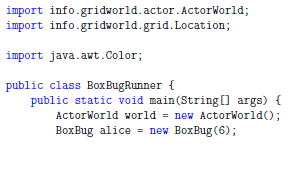
\includegraphics{A1}
	\\
	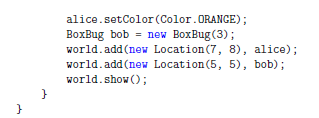
\includegraphics{A2}
	\\
	
	Semua yang terdapat pada code tersebut seharusnya terlihat familiar, dengan pengecualian untuk lokasi yang dimana ini merupakan bagian dari GridWorld dan mirip seperti java.awt.Point
	\newpage
	
	BoxBug.java memilki class yang mendifinisikan bagian dari BoxBug
	\\
	\\
	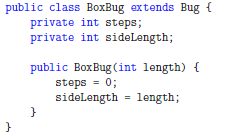
\includegraphics{B1}
	\\
	Baris pertama pada code tersebut menjelaskan bahwa class ini merupakan bagian dari Bug, yang berarti BoxBug merupakan salah satu jenis Bug.
	\\
	
	Lalu pada 2 baris berikutnya merupakan instance variables. Setiap Bug memiliki variables yang bernama sideLength, yang dapat diartikan sebagai ukuran box yang digambarkan, dan langkahnya, yang akan memantau berapa banyak langkah yang telah Bug lakukan.
	\\
	
	Baris berikutnya menjelaskan tentang Constructor yaitu metodee special yang berguna untuk membuat nilai awal pada instance variables. Ketika kamu membuat Bug dengan menggunakan new, java akan menggunakan constructor ini.
	\\
	
	Parameter untuk constructor ini adalah sideLength.
	\\
	
	Kelakuan dari Bug di kendalikan oleh metodee bernama act. Dibawah ini adalah metodee act untu BoxBug : 
	\\
	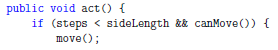
\includegraphics{C1}
	\\
	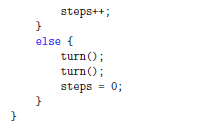
\includegraphics{C2}
	\\
	
	Jika BoxBug dapat bergerak, dan tidak mengambil angka yang dibutuhkan untuk setiap steps maka ia akan bergerak dan menambahkan steps setiap kali ia bergerak.
	\\
	
	Jika ia berhenti atau sudah berada pada kondisi akhir, maka ia berubah 90 derajat ke kanan dan kembari mereset steps ke 0.
	\\
	
	Jalankan programnya dan lihat apa yang dilakukan. Apakah kamu mendapatkan langkah yang seperti kamu inginkan?
	\\
	
	\section*{10.1 Termites}
	Saya menulis class yang bernama Termite yang merupakan bagian dari Bug dan menambahkan kemampuan untuk berinteraksi dengan flowers. Untuk menjalankannya, download file tersebut dan import ke dalam lokasi kamu membuat program tersebut : 
	\\
	
	\url{http://thinkapjava.com/code/Termite.java}
	\url{http://thinkapjava.com/code/Termite.gif}
	\url{http://thinkapjava.com/code/TermiteRunner.java}
	\url{http://thinkapjava.com/code/EternalFlower.java}
	\\
	
	Dikarenakan Termite merupakan bagian dari Bug, semua metode yang ada di Bug juga dapat dilakukan di dalam Termites. Tetapi Termites memiliki metode tambahan yang tidak dimiliki oleh Bug.
	\newpage
	
	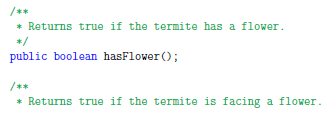
\includegraphics{D1}
	\\
	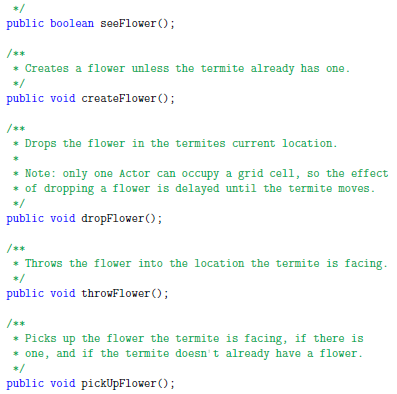
\includegraphics{D2}
	\\
	
	{\small Penjelasan Komentar}\\
	{\footnotesize comment 1 : Kembalikan True jika termite memiliki flower}\\
	{\footnotesize comment 2 : Kembalikan True jika termite bertemu dengan flower}\\
	{\footnotesize comment 3 : Buat flower kecuali termite sudah memiliki satu}\\
	{\footnotesize comment 4 : Jatuhkan flower di lokasi termites saat itu}\\
	{\footnotesize comment 5 : Lempar flower ke arah pandang termite}\\
	{\footnotesize comment 6 : Ambil flower dimana termite melihatnya, jika terdapat satu dan jika termite belum memiliki flower}\\
	\newpage
	
	Untuk beberapa metodee Bug menyediakan satu ketentuan dan Termite menyediakan yang lain dalam suatu kasus, metode yang dimiliki Termite akan mengesampingkan metode Bug.
	\\
	
	Untuk contohnya, ‘Bug.canMove’ mengembalikan True jika disana terdapat flower di lokasi berikutnya, maka Bugs juga dapat menginjak flowers. Termite.canMove ajan mengembalikan False jika disana terdapat object di lokasi beriktunya, maka Termite dapat melakukan hal yang berbeda dari Bug.
	\\
	
	Dalam contoh lain, Termites memiliki versi dari langkah yang dia ambil menggunakan integer sebagai parameter. Yang akhirnya Termites memiliki ‘randomTurn’. Yaitu dapat berbalik 45 derajat ke kiri atau kanan secara acak.
	\\
	
	Ini code dari TermiteRunner.java : 
	\\
	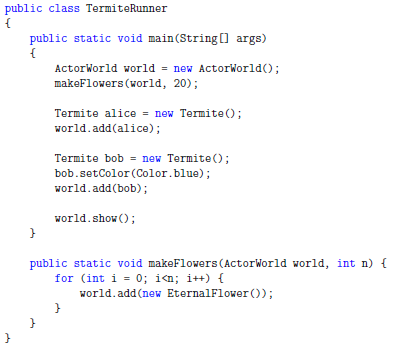
\includegraphics{E1}
	\\
	
	Semua yang ada di dalam code tersebut mungkin terlihat tidak asing. TermiteRunner membuat ActorWorld dengan 20 EternalFlowers dan 2 Termites.
	\\
	
	EternalFlower adalah bunga yang dapat mengesampingkan act jadi flowers tidak terlihat menggelap.
	\\
	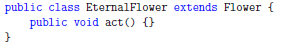
\includegraphics{F1}
	\\
	
	Jika kamu menjalankan TermiteRunner.java kamu akan melihat 2 termites berjalan secara acak diantara flowers.
	\\
	
	MyTermite.java mendemonstrasikan metode yang berinteraksi dengan flowers. Ini salah definisi dari class tersebut : 
	\\
	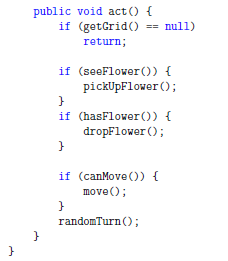
\includegraphics{G1}
	\\
	
	MyTermite merupakan class bagian dari Termite dan mengesampingkan act. If MyTermite melihat flower, ia akan mengambilnya. Jika ia memiliki flower, maka jatuhkan bunganya.
	\\
	
	\section*{10.2 Langton's Termite}
	Langton’s Ant adalah model sederhana dari bagaimana ant bertindak yang menampilkan tindakan yang sangat complex. The Ant tinggal di dalam grid seperti GridWorld dimana setiap cell dalah putih atau hitam. The Ant bergerak menurut perintah tersebut : 
	\\
	
	\begin{itemize}
		\item Jika The Ant ada di cell yang berwarna putih, maka ia akan merubah arah ke kanan, membuat cell tersebut menjadi berwarna hitam dan maja kedepan.
		\item Jika The Antada di cell yang berwarna hitam, maka ia akan merubah arah ke kiri, dan membuat cell tersebut menjadi berwarna putih dan maju kedepan.
	\end{itemize}
	\newpage
	
	Dikarenankan peraturan tersebut sangatlah sederhana, kamu mungkin mengira bahwa The Ant akan melakukan sesuatu yang sederhana seperti membuat kotak atau mengulang pola sederhana yang sama. Tetapi dimulai dari semua cell yang berwarna putih, The Ant membuat lebih dari 10,000 langkah yang acak sebelum berubah ke perulangan yang sama sebanyak 104 langkah.
	\\
	
	Kamu dapat membaca lebih banyak dari Langton’s Ant di \\
	\url{http://en.wikipedia.org/wiki/Langtin_ant}
	\\
	
	Ini tidak mudah untuk mengimplementasikan Langton’s Ant di dalam GridWorld karena kita dapat merubah warna dari cells. Sebagai alternatif kita dapat menggunakan Flowers untuk menandakan cells, tetapi kita tetap tidak dapat membuat Ant dan Flower berada di dalam cell yang sama maka dari itu kita tidak dapat mengimplementasikan aturan The Ant secara tepat.
	\\
	
	Sebagai gantiya kita akan membuat apa yang disebut LangtonTermite, dimana menggunakan ‘seeFlower’ untuk mengecek apakah terdapat Flower di cell berikutnya, ‘pickUpFlower’ untuk mengambil dan ‘throwFlower’ untuk menaruh Flower di cell berikutnya. Kamu mungkin ingin membaca code dari metode tersebut untuk meyakinkan bahwa kamu mengetahui apa yang mereka lakukan.
	\\
	
	\section*{10.3 Latihan}
	\subsection*{Latihan 10.1}
	Sekarang kamu sudah cukup memahami untuk mengerjakan latihan yang ada pada pedoman siswa, Part 2. Kerjakan latihan tersebut, dan kembali untuk mendapatkan hal yang lebih.
	\\
		
	\subsection*{Latihan 10.2}
	Tujuan dari latihan ini adalah untuk mengetahui tingkah laku dari Termites yang berinteraksi dengan Flowers.
	\\
	
	Ubah TermiteRunner.java untuk membuat MyTermites untuk menggantikan Termites. Lalu jalankan lagi. MyTermites harus dapat bergerak secara acak, dan membawa bunga. Total dari bunga harus sama(termasuk yang dapat MyTermites bawa)
	\newpage
	
	Di dalam ‘Termites, Turtles and Traffic Jams’, Mitchell Resnick menjelaskan tindakan sederhana yang dilakukan oleh termite sebagai berikut : 
	
	\begin{itemize}
		\item Jika dia melihat flower, maka ambil. Kecuali dia sudah memiliki bunga tersebut dalam hal tersebut maka jatuhkan yang kamu punya.
		\item Maju kedepan jika dia bisa.
		\item Belok kiri atau kanan secara acak.
	\end{itemize}
	
	Ubah MyTermite.java untuk mengimplementasikan model tersebut. Menurut kamu efek apa yang akan terjadi pada tingkah laku dari MyTermites?
	\\
	
	Coba lagi, lalu selanjutya, total flower yang ada tidak berubah namun secara beberapa waktu the flowers akan muncul dalam tumpukan yang kecil, terkadang hanya satu.
	\\
	
	Tingkah laku ini ada di dalam ‘an emergent property’, yang dapat kamu baca di \url{http://en.wikipedia.org/wiki/Emergence}. MyTermites mengikuti peraturan sederhana dengan hanya menggunakan informasi berskala kecil, tetapi dengan hasil organisasi dengan skala yang besar.

	Bereksperimenlah dengan peraturan yang berbeda dan lihat efek apa yang akan terjadi pada sistem tersebut. Perubahan kecil dapat menghasilkan hasil yang tidak terduga.

	\subsection*{Latihan 10.3}
	\begin{enumerate}
		\item Buat salinan dari Termite.java dengan nama LangtinTermite dan salinan dari TermiteRunner.java dengan nama LangtonRunner.java ubah file tersebut sehingga classnya sama dengan file dan juga LangtinRunner membuat LangtonTermite.
		\item Jika kamu membuat file bernama LangtonTermite.gif, GridWorld menggunakan itu untuk menampilkan Termite kamu, kamu dapat mengunduh gambar-gambar serangga yang bagus dari \url{http://www.cksinfo.com/animals/insects/realisticdrawings/index.html}. Untuk mengubah file tersebut ke dalam format GIF, kamu dapat menggunakan aplikasi seperti ImageMagick.
		\item Ubah act untuk mengimplementasikan peraturan yang mirip dengan Lanton’s Ant. Coba bereksperimantasilah dengan berbagai macam peraturan dan dengan belokan 45 dan 90 derajat. Cari aturan yang paling memiliki banyak langkah sebelum Termite memulai pengulangan langkah.
		\item Untuk membuat Termite ruangan yang cukup besar, kamu dapat membuat gridnya lebih besar atau ubah ke UnboudedGrid.
		\item Buat lebih dari satu LangtonTermite dan lihat bagaimana mereka berinteraksi.
	\end{enumerate}
	
	
\end{document}
\chapter{Membuat Objek}
\section{Definisi Class dan Tipe Objek}

Kembali pada Bagian 1.5 ketika kita mendefinisikan kelas Hello, kita juga membuat jenis objek bernama Hello. Kita tidak menciptakan variabel dengan tipe Hello, dan kami tidak membuat objek Hello, tapi kita bisa buat !

Contoh yang tidak masuk akal, ketika tidak ada alasan untuk membuat objek Hello, dan itu tidak akan berbuat lebih jika kita lakukan. Dalam bab ini, kita akan melihat definisi Class yang menciptakan jenis objek yang berguna.

Berikut adalah hal yang paling penting dalam bab ini:

\textbullet  Mendefinisikan Class baru juga menciptakan jenis objek baru dengan nama yang sama.

\textbullet  Sebuah definisi Class seperti template untuk objek, menentukan apa variabel misalnya memiliki objek dan metode apa yang dapat beroperasi pada method.

\textbullet  Setiap objek memiliki beberapa jenis objek.

\textbullet  Ketika kamu membuat sebuah objek baru, Java memanggil method khusus yang disebut constructor untuk menginisialisasi variabel instance. Kamu dapat memberikan satu atau lebih konstruktor sebagai bagian dari definisi kelas.

\textbullet  Method yang dapat beroperasi pada tipe yang dapat didefinisikan dalam class tersebut.

Berikut adalah beberapa masalah tentang syntax pada definisi class:

\textbullet Nama Class, harus diawali dengan huruf kapital, yang membantu membedakan apakah itu tipe primitif dan nama variabel.

\textbullet Kamu biasanya menempatkan satu definisi kelas di setiap file, dan nama file harus sama dengan nama kelas, dengan .java akhir nama file. Sebagai contoh, Class Time didefinisikan dalam file bernama Time.java.

\textbullet Dalam program apapun, satu kelas yang ditunjuk sebagai class awal. Class awal harus berisi sebuah method main (Method Utama), yang mana program tersebut akan dieksekusi. Kelas-kelas lain mungkin memiliki method main, tapi itu tidak akan dieksekusi.

Dengan masalah tersebut. Mari lihat contoh pada Class Time(Waktu).

\section{Waktu}

Sebuah motivasi untuk menciptakan jenis objek adalah untuk merangkum data dalam suatu objek yang dapat dilakukan sebagai satu kesatuan. Kita telah melihat dua jenis seperti ini, titik dan kotak.

Contoh lain, yang kita akan menerapkan diri kita sendiri, adalah waktu, yang merepresentasikan waktu dalam hari. Data disimpan dalam sebuah objek Waktu adalah satu jam, satu menit, dan sejumlah detik. Karena setiap objek Waktu mengandung data jam, menit, dan detik, maka kita perlu variabel.

Langkah pertama adalah untuk menentukan jenis setiap variabel. Jelas bahwa jam dan menit harus bilangan bulat (int). Untuk lebih menarik, maka kita buat detik menggunakan double.

Contoh variabel dideklarasikan di awal definisi class, seperti berikut
\newline
class Waktu \textbraceleft \newline
	int jam, menit; \newline
	double detik; \newline
\textbraceright

Dengan sendirinya, kode diatas merupakan definisi class. Setelah mendeklarasikan variabel, langkah selanjutnya yaitu menentukan konstruktor untuk class baru.


\section{Konstruktor}

Konstruktor adalah inisialisasi dari variabel. Sintaks untuk konstruktor mirip seperti method lain,tapi dengan tiga pengecualian: \newline

\textbullet Nama konstruktor sama dengan nama class. \newline

\textbullet Konstruktor tidak memiliki nilai kembali (return type). \newline

\textbullet Keyword statis dihilangkan. \newline

Kita berikan contoh untuk class Waktu: \newline

public Waktu()\textbraceleft \newline
	this.jam = 0; \newline
	this.menit = 0; \newline
	this.detik = 0.0; \newline
\textbraceright	


Mana yang kamu harapkan untuk melihat return type, antara public dan Waktu, tidak ada bukan ?. Itulah cara kita (dan compiler) dapat memberitahu bahwa ini adalah sebuah konstruktor.

Konstruktor tidak akan mengambil argumen. Setiap baris dari konstruktor menginisialisasi sebuah variabel untuk nilai default. Nama ini adalah kata kunci khusus yang mengacu pada objek yang kita ciptakan. Kamu dapat menggunakan ini dengan cara yang sama kamu gunakan untuk nama benda lainnya. Sebagai contoh, Kamu dapat membaca dan menulis variabel contoh ini, dan Kamu dapat melewati ini sebagai argumen untuk method lain.

Tapi kamu tidak menyatakan ini dan kamu tidak dapat membuat sebuah tugas untuk itu. ini dibuat oleh sistem, yang harus kamu lakukan adalah menginisialisasi variabel nya.

\section{Konstruktor (Lanjutan)}

Konstruktor dapat overload, seperti method lain, yang berarti bahwa kamu dapat memberikan beberapa konstruktor dengan parameter yang berbeda. Java tahu yang konstruktor dengan cara mencocokkan argumen baru dengan parameter konstruktor.

Umum untuk memiliki satu konstruktor yang tidak memiliki argumen, dan satu konstruktor yang mengambil daftar parameter identik dengan daftar variabel misalnya. Sebagai contoh:
\newline
public Waktu (int jam, int menit, double detik)\textbraceleft \newline
	this.jam = jam; \newline
	this.menit = menit; \newline
	this.detik = detik; \newline
\textbraceright \newline

Nama dan jenis parameter akan sama dengan nama dan jenis variabel. Semua konstruktor tidak menyalin informasi dari parameter untuk variabel.

Jika kamu melihat dokumentasi untuk point dan kotak, kamu akan melihat bahwa kedua kelas menyediakan konstruktor seperti ini. Overloading konstruktor menyediakan fleksibilitas untuk membuat objek pertama dan kemudian mengisi kekosongan, atau untuk mengumpulkan semua informasi sebelum membuat objek.

Ini mungkin tidak tampak menarik. Menulis konstruktor adalah membosankan, prosesnya selalu mekanis. Setelah kamu telah menulis dua variabel, Kamu akan menemukan bahwa kamu dapat menulis dengan cepat hanya dengan melihat daftar variabel misalnya.

\section{Membuat Objek Baru}

Meskipun konstruktor terlihat seperti method, Kamu tidak pernah memanggil mereka secara langsung. Sebaliknya, ketika kamu memanggil konstruktor baru, dimulai dari sistem mengalokasikan ruang untuk objek baru baru kemudian kamu akan memanggil konstruktor.

Program berikut menunjukkan dua cara untuk membuat dan menginisialisasi objek Waktu:
\newline
class Waktu \textbraceleft \newline
	int jam, menit; \newline
	double detik; \newline
\newline	
	public Waktu()\textbraceleft \newline
		this.jam = 0; \newline
		this.menit = 0; \newline
		this.detik = 0.0; \newline
	\textbraceright \newline
\newline
	public Waktu(int jam, int menit, double detik)\textbraceleft \newline
	this.jam = jam; \newline
	this.menit = menit; \newline
	this.detik = detik; \newline
	\textbraceright \newline
\newline
	public static void main(String[] args)\textbraceleft \newline
	Waktu w1 = new Waktu(); \newline
	w1.jam = 11; \newline
	w1.menit = 8; \newline
	w1.detik = 3.14159; \newline
	System.out.println(w1); \newline
\newline
	Waktu w2 = new Waktu(11, 8, 3.14159); \newline
	System.out.println(w2); \newline
	\textbraceright \newline
\textbraceright

Dalam method main, pertama kali kita memanggil objek baru, kita tidak memberikan sebuah argumen, sehingga Java memanggil konstruktor pertama. Beberapa baris berikutnya baru memberikan nilai pada variabel.

Pada saat yang kedua kita panggil objek baru, kita memberikan argumen yang sesuai dengan parameter konstruktor kedua. Ini cara menginisialisasi variabel misalnya lebih ringkas dan sedikit lebih efisien, tetapi bisa sulit untuk dibaca, karena tidak jelas mana nilai yang ditugaskan untuk variabel misalnya.

\section{Mencetak Objek}

Hasil output pada program sebelumnya yaitu :
\newline
Waktu@80cc7c0 \newline
Waktu@80cc807 \newline

Ketika Java mencetak nilai dari user-defined, mencetak nama jenis dan heksadesimal khusus (basis 16) kode yang unik untuk setiap objek. Kode ini tidak berarti dalam dirinya sendiri; pada kenyataannya, itu dapat bervariasi dari mesin ke mesin dan bahkan dari compiler untuk menjalankan. Tetapi dapat berguna untuk debugging, jika kamu ingin melacak objek individu.

Untuk mencetak objek dalam cara yang lebih berarti untuk pengguna, Kamu dapat menulis sebuah metode yang disebut sesuatu seperti cetakWaktu:
\newline
public static void cetakWaktu(Waktu w)\textbraceleft \newline
	System.out.println(w.jam + ":" + w.menit + ":" + w.detik); \newline
\textbraceright

Output dari method ini, jika kita beranggapan baik w1 atau w2 sebagai argumen, outputnya adalah 11: 8: 3.14159. Meskipun ini dikenali sebagai waktu, tidak cukup dalam format standar. Sebagai contoh, jika jumlah menit atau detik kurang dari 10, kita mungkin ingin menghapus bagian desimal dari detik. Dengan kata lain, kita ingin sesuatu seperti 11:08:03.

Dalam kebanyakan bahasa, ada cara sederhana untuk mengontrol output format untuk nomor. Di Javaa tidak ada cara sederhana.

Java menyediakan sebuah mekanisme untuk mencetak hal-hal seperti format waktu dan tanggal, dan juga untuk menafsirkan masukan apa yang di format. Kamu dapat melihat dokumentasi untuk class Tanggal dalam paket java.util.

\section{Operasi pada Objek}

Dalam bagian berikutnya, terdapat 3 macam metode yang beroperasi pada objek : \newline
\textbullet \textbf{Pure Function} : Mengambil objek sebagai argumen tetapi tidak dapat memodifikasi. Nilai return yaitu baik objek primitif atau objek baru dibuat di dalam metode. \newline
\textbullet \textbf{Modifier} : Mengambil objek sebagai argumen dan dapat dimodifikasi beberapa atau semua yang terdapat pada modifier tersebut. bahkan nilai return void. \newline
\textbullet \textbf{Fill-in Method} : Salah satu objek yang kosong, Objek akan diisi oleh method itu sendiri. Secara teknis, fill-in method  adalah tipe modifier. \newline

\section{Pure Functions}

Sebuah method dianggap sebagai fungsi murni jika hasilnya bergantung hanya pada argumen, dan tidak memiliki efek lainnya seperti memodifikasi sebuah argumen atau mencetak sesuatu. Satu-satunya hasil fungsi murni adalah nilai kembali.

Salah satu contoh adalah isAfter, yang membandingkan dua Waktu dan mengembalikan tipe boolean yang menunjukkan apakah operan pertama datang setelah kedua:
\newline
public static boolean isAfter(Waktu w1, Waktu w2)\textbraceleft \newline
	if (w1.jam \textgreater w2.jam) \newline
		return ture; \newline
	if (w1.jam \textless w2.jam) \newline
		return false; \newline
\newline
	if (w1.menit \textgreater w2.menit) \newline
		return true; \newline
	if (w1.menit \textless w2.menit) \newline
		return false; \newline
\newline
	if (w1.detik \textgreater w2.detik) \newline
		return false; \newline
\textbraceright \newline
\newline
Contoh kedua adalah tambahWaktu, yang menghitung jumlah dua kali. Sebagai contoh, jika 09:14:30, dan membuat roti membutuhkan 3 jam dan 35 menit, Kamu bisa menggunakan tambahWaktu untuk mencari tahu ketika roti akan dilakukan.

Berikut ini adalah draft kasar dari method ini yang tidak benar:
\newline \newline
public static Waktu tambahWaktu(Waktu w1, Waktu w2)\textbraceleft \newline
	Waktu tambah = new Waktu(); \newline
	tambah.jam = w1.jam + w2.jam; \newline
	tambah.menit = w1.menit + w2.menit; \newline
	tambah.detik = w1.detik + w2.detik \newline
	return tambah; \newline
\textbraceright \newline \newline
Meskipun method ini mengembalikan sebuah objek Waktu, itu bukan sebuah konstruktor. Kamu harus kembali dan membandingkan sintaks dari method seperti ini dengan sintaks konstruktor, karena mudah untuk mendapatkannya.

Berikut adalah contoh bagaimana menggunakan method ini. Jika currentTime berisi waktu saat ini dan breadTime mengandung jumlah waktu yang diperlukan untuk membuat roti, maka kamu bisa menggunakan tambahWaktu untuk mencari tahu ketika roti akan dilakukan.
\newline
Waktu currentTime = new Waktu(9, 14, 30.0); \newline
Waktu breadTime = new Waktu(3, 35, 0.0); \newline
Waktu doneTime = tambahWaktu(currentTime, breadTime); \newline
cetakWaktu(doneTime); \newline

Output dari program ini adalah 12: 49: 30.0, yang benar. Di sisi lain, ada kasus di mana hasilnya tidak benar. Dapatkah Anda memikirkan yang tidak benar ?

Masalahnya adalah bahwa method ini tidak menangani kasus-kasus di mana jumlah detik atau menit menambahkan hingga lebih dari 60. Dalam hal ini, kita harus "membawa" detik-detik ekstra ke dalam kolom menit, atau menit ekstra ke dalam kolom jam .

Berikut adalah versi method yang sudah dikoreksi.

\newline
public static Waktu tambahWaktu(Waktu w1, Waktu w2)\textbraceleft \newline
	Waktu tambah = new Waktu(); \newline
	tambah.jam = w1.jam + w2.jam; \newline
	tambah.menit = w1.menit + w2.menit; \newline
	tambah.detik = w1.detik + w2.detik; \newline
\newline
	if(tambah.detik \textgreater = 60.0)\textbraceleft \newline
		tambah.detik -= 60; \newline
		tambah.menit += 1; \newline
	\textbraceright \newline
\newline
	if (tambah.menit \textgreater = 60)\textbraceleft \newline
		tambah.menit -= 60; \newline
		tambah.jam += 1; \newline
	\textbraceright \newline
\textbraceright \newline
Meskipun benar, ada cara alternatif yang jauh lebih pendek.

Kode ini menunjukkan dua operator, kita belum pernah melihat sebelumnya, + = dan - =. Operator ini menyediakan cara ringkas untuk kenaikan dan penurunan variabel. Mereka mirip dengan ++ dan --, \newline kecuali \newline (1) variabel yang bekerja yaitu int, dan \newline (2) jumlah selisih tidak harus 1. Pernyataan sum.second - = 60,0; setara dengan sum.second = sum.second - 60; \newline
\section{Modifiers}

Sebagai contoh pada modifier, increment, yang menambahkan jumlah detiks ke objek Waktu. Sekali lagi, konsep dari method ini terlihat seperti berikut :
\newline
public static void increment(Waktu waktu, double detiks)\textbraceleft \newline
	waktu.detik += detik2; \newline
\newline
	if(waktu.detik \textgreater = 60.0)\textbraceleft \newline
		waktu.detik -= 60.0; \newline
		waktu.menit += 1; \newline
	\textbraceright \newline
\newline
	if(waktu.menit \textgreater = 60)\textbraceleft \newline
		waktu.menit -= 60; \newline
		waktu.jam += 1; \newline
	\textbraceright \newline
\textbraceright \newline

Baris pertama melakukan operasi dasar; sisanya berkaitan dengan kasus yang sama yang kita lihat sebelumnya.

Apakah method ini sudah benar? Apa yang terjadi jika argumen detiks jauh lebih besar dari 60? Dalam hal ini, tidak cukup untuk mengurangi 60 sekali; kita harus terus melakukannya sampai detiks di bawah 60. Kita dapat melakukan itu dengan mengganti pernyataan dengan pernyataan sementara:

\newline

public static void increment(Waktu waktu, double detiks)\textbraceleft \newline
	waktu.detik += detiks; \newline
\newline
	while(waktu.detik \textgreater = 60.0)\textbraceleft \newline
		waktu.detik -= 60.0; \newline
		waktu.menit += 1; \newline
	\textbraceright \newline
\newline
	while(waktu.menit \textgreater = 60)\textbraceleft \newline
		waktu.menit -= 60; \newline
		waktu.jam += 1; \newline
	\textbraceright \newline
\textbraceright \newline

Solusi ini benar, tetapi tidak sangat efisien. Dapatkah kamu memikirkan solusi yang tidak memerlukan iterasi?

\section{Fill-in Methods}

Untuk menciptakan objek baru setiap kali tambahIsiWaktu dipanggil, kita bisa meminta untuk memberikan sebuah objek di mana tambahIsiWaktu menyimpan hasilnya. Bandingkan dengan versi sebelumnya:
\newline
public static void tambahIsiWaktu(Waktu w1, Waktu w2, Waktu tambah)\textbraceleft \newline
	tambah.jam = w1.jam + w2.jam; \newline
	tambah.menit = w1.menit + w2.menit; \newline
	tambah.detik = w1.detik + w2.detik; \newline
\newline
	if(tambah.detik \textgreater = 60.0)\textbraceleft \newline
		tambah.detik -= 60.0; \newline
		tambah.menit += 1; \newline
	\textbraceright \newline
\newline
	if(tambah.menit \textless = 60)\textbraceleft \newline
		tambah.menit -= 60; \newline
		tambah.jam += 1; \newline
	\textbraceright \newline
\textbraceright \newline
Hasilnya disimpan dalam variabel tambah, sehingga void merupakan return typenya.

Modifiers dan fill-in method merupakan yang efisien karena mereka tidak perlu membuat objek baru. Tapi mereka lebih sulit untuk mengisolasi bagian dari program; dalam skala proyek besar mereka dapat menyebabkan kesalahan yang sulit untuk menemukan / mencari data.

Pure functions dapat membantu mengelola kompleksitas proyek-proyek besar, sebagian dengan membuat beberapa jenis kesalahan, dan karena hasil dari pure functions hanya bergantung pada parameter, mungkin ada cara lain untuk mempercepat mereka dengan menyimpan hasil sebelumnya dihitung.
\newline
\section{Perencanaan dan Pengembangan pada Incremental}

Dalam bab ini akan ditunjukkan proses pengembangan program yang disebut prototyping. Untuk setiap method, kalian akan menulis draft kasar yang dilakukan dalam perhitungan dasar, kemudian diuji pada beberapa kasus, kemudian mengoreksi apa yang kurang.

Pendekatan ini bisa efektif, tetapi dapat menyebabkan kode yang tidak terlalu rumit, karena berhubungan dengan banyak kasus khusus dan tidak dapat diandalkan karena sulit untuk meyakinkan diri sendiri bahwa kamu telah menemukan sebuah kesalahan.

Sebuah alternatif untuk mencari wawasan ke dalam suatu masalah yang dapat membuat pemrograman jauh lebih mudah. Dalam hal ini wawasan adalah bahwa waktu adalah benar-benar angka tiga digit dalam basis 60! Yang kedua adalah menit "60 kolom", dan jam adalah "3600 kolom ."

Ketika kita menulis tambahWaktu dan increment, secara efektif dapat melakukan penambahan pada basis 60, itulah sebabnya mengapa kita harus " membawa dari satu kolom ke yang berikutnya.

Pendekatan lain untuk seluruh masalah adalah untuk mengkonversi Waktu menjadi double dan mengambil keuntungan dari fakta bahwa komputer sudah tahu bagaimana melakukan aritmatika dengan double. Berikut adalah metode yang mengubah waktu menjadi double:

\newline

public static double converttoSeconds(Waktu w)\textbraceleft \newline
	int menit = w.jam * 60 + t.menit; \newline
	double detik = menit * 60 + w.detik; \newline
	return detik; \newline
\textbraceright \newline

Sekarang semua yang kita butuhkan adalah cara untuk mengkonversi dari double untuk objek Waktu. Kita bisa menulis sebuah metode untuk melakukannya, tapi mungkin lebih masuk akal untuk menulis sebagai konstruktor:

\newline
public Waktu(double detik)\textbraceleft \newline
	this.jam = (int)(detik / 3600.0); \newline
	detik -= this.jam * 3600.0; \newline
	this.menit = (int)(detik / 60.0); \newline
	detik -= this.menit * 60; \newline
	this.detiks = detik; \newline
\textbraceright \newline

Konstruktor ini sedikit berbeda dari yang lain; melibatkan beberapa kalkulasi bersama untuk variabel.

Kamu mungkin harus berpikir untuk meyakinkan diri sendiri bahwa teknik yang digunakan untuk mengkonversi dari satu basis ke yang lain harus benar. Tapi setelah kamu yakin, kita dapat menggunakan metode ini untuk menulis ulang tambahWaktu:
\newline
public static Waktu tambahWaktu(Waktu w1, Waktu w2)\textbraceleft \newline
	double detik = converttoSeconds(w1) + converttoSeconds(w2); \newline
	return new Waktu(detik); \newline
\textbraceright \newline

Ini lebih pendek dari versi yang asli, dan jauh lebih mudah untuk menunjukkan bahwa itu adalah benar (dengan asumsi, seperti biasa, bahwa method yang dipanggil itu benar). Sebagai latihan, tulis ulang increment dengan cara yang sama.

\section{Peraturan Umum}

Dalam beberapa hal mengkonversi dari basis 60 ke basis 10 adalah hal yang lebih sulit daripada hanya berurusan dengan waktu. Konversi basis lebih abstrak; intuisi kita untuk menangani waktu harus lebih baik.

Tetapi jika kita memiliki wawasan untuk mengakali sebagai basis 60 angka, dan membuat investasi menulis metode konversi (convertToSeconds dan konstruktor pihak ketiga), kita mendapatkan sebuah program yang lebih pendek, lebih mudah dibaca dan dapat debug, dan lebih handal.

Hal ini juga lebih mudah untuk menambahkan fitur. Bayangkan jika kita kurangi dua kali untuk mencari durasi antara dua kali tersebut. Menggunakan metode konversi akan jauh lebih mudah.

Terkadang jika masalah lebih sulit membuat lebih mudah (kasus khusus yang lebih sedikit, lebih sedikit kesempatan untuk salah).

\section{Algoritma}

Ketika kamu menulis sebuah solusi umum untuk masalah dalam sebuah class, maka akan muncul solusi yang spesifik yang mengacu pada satu masalah, kamu akan menuliskannya pada sebuah algoritma. 

Pertama, pertimbangkan beberapa hal yang bukan algoritma. Ketika Kamu belajar untuk memperbanyak nomor satu digit, Kamu mungkin menghafal tabel perkalian. Akibatnya, Kamu hafal 100 solusi spesifik, sehingga pengetahuanmu bukan secara algoritmik.

Tetapi jika kamu malas, kamu mungkin belajar beberapa trik. Misalnya, untuk produk dari n dan 9, Kamu dapat menulis n - 1 sebagai digit pertama dan 10 - n sebagai digit kedua. Trik ini adalah solusi umum untuk mengalikan nomor satu digit dengan 9. Itu adalah suatu algoritma!

Demikian pula, teknik yang kamu pelajari untuk penambahan dengan membawa, pengurangan dengan meminjam. Salah satu karakteristiknya algoritma adalah bahwa algoritma tidak memerlukan kecerdasan apapun untuk melaksanakannya. Algoritma adalah  Sebuah instruksi untuk menyelesaikan sebuah masalah dalam class oleh proses mekanik.

Menurut pendapat saya, memalukan bahwa siswa menghabiskan begitu banyak waktu di sekolah belajar untuk mengeksekusi algoritma. Di sisi lain, proses merancang algoritma yang menarik, intelektual yang menantang, dan bagian sentral dari apa yang kita sebut pemrograman.

Beberapa hal yang dilakukan orang secara alami, tanpa kesulitan adalah yang paling sulit untuk mengekspresikan algoritma. Memahami bahasa alami adalah contoh yang baik. Kita semua melakukannya, tapi sejauh ini belum ada yang mampu menjelaskan bagaimana kita melakukannya, setidaknya tidak dalam bentuk algoritma.

Segera Kamu akan memiliki kesempatan untuk merancang algoritma sederhana untuk berbagai masalah. 

\section{Istilah - Istilah}

\textbullet \textbf{Class} : Sebelumnya, sudah dijelaskan bahwa class kumpulan dari beberapa method. Dalam Bab ini kita belajar bahwa definisi class yaitu sebagai template (klise) untuk tipe objek yang baru. \newline

\textbullet \textbf{Instance} : Sebuah member dalam class. Setiap objek pada instance merujuk pada beberapa class. \newline

\textbullet \textbf{Konstruktor} : Method spesial yang menginisialisasikan variabel instance pada sebuah objek konstruktor yang baru. \newline

\textbullet \textbf{Class Awal} : Class yang berisi method utama dimana program tersebut akan dieksekusi. \newline

\textbullet \textbf{Pure Function} : Method yang hasilnya bergantung pada parameter dan tidak memiliki efek lain selain pengembalian nilai. \newline

\textbullet \textbf{Modifier} : Method yang dapat mengganti satu atau beberapa objek yang dapat menerima parameter dan kebanyakan mengembalikkan nilai kosong. \newline

\textbullet \textbf{Fill-in Method} : Tipe Method yang mengambil objek kosong sebagai parameter dan diisi sebagai variabel instance sebagai contoh dapat pengembalian nilai. \newline

\textbullet \textbf{Algoritma} : Sebuah instruksi untuk menyelesaikan sebuah masalah dalam class oleh proses mekanik. \newline


\section{Latihan}

Latihan 11.1. Dalam permainan papan Scrabble, setiap kotak berisi huruf, yang digunakan untuk mengeja kata-kata, dan nilai, yang digunakan untuk menentukan nilai dari kata-kata.
\newline
1. Tulis definisi untuk kelas bernama Ubin yang mewakili ubin pada Scrabble. \newline
Variabel harus karakter berhuruf dan integer.
\newline \newline
2. Tulis konstruktor yang mengambil parameter berhuruf , nilai dan menginisialisasi pada variabel.
\newline \newline
3. Tulis method bernama printTile yang mengambil objek Tile sebagai parameter dan mencetak variabel.
\newline \newline
4. Tulis method bernama testTile yang menciptakan objek Tile dengan huruf Z dan nilai 10, kemudian mgunakan printTile untuk mencetak hasil dari objek.
\newline \newline
Inti dari latihan ini adalah untuk melatih pada bagian mekanismenya untuk menciptakan kelas baru dan kode yang tes tersebut.
\newline \newline
Latihan 11.2. Tulis definisi kelas untuk Tanggal, jenis objek yang membandingkan tiga bilangan bulat, tahun, bulan dan hari. Kelas ini harus menyediakan dua konstruktor. Yang pertama harus ada parameter. Kedua harus mengambil parameter bernama tahun, bulan dan hari, dan menggunakannya untuk menginisialisasi variabel.
\newline \newline
Tulis method utama yang menciptakan objek Tanggal bernama ulangTahun. Objek baru harus berisi tanggal lahir kamu. Kamu dapat menggunakan salah satu konstruktor.
\newline \newline
Latihan 11.3. Bilangan rasional adalah angka yang dapat direpresentasikan sebagai rasio dua bilangan bulat. Misalnya, 2/3 adalah bilangan rasional, dan Kamu dapat memikirkan 7 sebagai bilangan rasional dengan implisit 1 di penyebut. Untuk tugas ini, Kamus akan menulis sebuah definisi kelas untuk bilangan rasional.
\newline \newline
1. Buat program baru yang disebut Rational.java yang mendefinisikan kelas bernama Rational. Sebuah objek Rational harus memiliki dua contoh bilangan bulat (integer) untuk menyimpan pembilang dan penyebut.
\newline \newline
2. Tulis konstruktor yang tidak mengambil argumen dan yang menentukan dari pembilang ke 0 dan penyebut untuk 1.
\newline \newline
3. Tulis method printRational yang mengambil benda Rasional sebagai argumen dan mencetaknya.
\newline \newline
4. Tulis method main yang menciptakan objek baru dengan tipe Rasional, dan membuat variabel misalnya untuk beberapa nilai, dan mencetak objek.
\newline \newline
5. Pada tahap ini, Kamu sudah memiliki program yang dapat diuji. Ujilah dan jika perlu, debug itu.
\newline \newline
6. Tulis konstruktor yang kedua untuk kelas kamu yang membutuhkan dua argumen dan gunakan untuk menginisialisasi variabel.
\newline \newline
7. Tulis method yang disebut negate yang mengembalikkan bilangan rasional. Method ini harus modifier. Tambahkan baris main untuk menguji method baru. 
\newline \newline
8. Tulis method yang disebut invert yang mengembalikkan nomor dengan swapping pembilang dan penyebut. Tambahkan baris main untuk menguji method baru.
\newline \newline
9. Tulis method yang disebut toDouble yang mengubah bilangan rasional menjadi bilangan decimal (double) dan mengembalikan hasilnya. Method ini adalah pure functions, tidak dapat memodifikasi objek. Seperti biasa, uji method tersebut.
\newline \newline
10. Tulis modifier bernama reduce yang mengurangi jumlah bilangan rasional untuk persyaratan terendah dengan mencari pembagi terbesar dari pembilang dan penyebut. Method ini harus menjadi pure functions; tidak harus memodifikasi variabel  dari objek di mana ia dipanggil.
\newline \newline
11. Tulis method yang disebut add yang mengambil dua angka Rational sebagai argumen dan mengembalikan sebuah objek Rational baru. return objek harus berisi jumlah dari argumen tersebut.
\newline \newline
Ada beberapa cara untuk menambahkan fraksi. Kamu dapat menggunakan salah satu yang kamu inginkan, tetapi kamu harus memastikan bahwa hasil dari operasi berkurang sehingga pembilang dan penyebut tidak memiliki pembagi umum (selain 1).
\newline \newline
Tujuan dari latihan ini adalah untuk menulis sebuah definisi kelas yang meliputi berbagai method, termasuk konstruktor, modifiers dan pure functions.
%%%%%%%%%%%%%%%%%%%%%%%%%%%%%%%%%%%%%%%%%%%%%%%%%%%%%%%
\backmatter
%\include{glossary}

\printindex
\end{document}